\chapter{Last Year Review}

As our project is a continuation of work previously developed by another 4th year group, we must review the previous groups work and highlight any potential issues that could prove troublesome or helpful/useful in the completion of our system. The Social network analysis tool developed by the group from the previous year was a very well presented and constructed program. The main goals of this software was to allow a user to study and implement various algorithms across varying forms of social network. The interface was intended to handle extremely large amounts of local or remote data seamlessly. Focussing on the collapse of the Enron company, they modelled the communication interaction between colleagues at the company and conducted extensive research into the network model developed from the acquired data. 

The Design of the social network analysis tool was split into 7 major sections which are the:

\begin{itemize}
\item Database
\item Database Proxy
\item Network model
\item Algorithms
\item Graphical User interface
\item Batch processing component
\end{itemize}

These components connected into the system as shown in the image \ref{fig:previous-review-system-diagram}.

\begin{figure}[htbp]
	\centering
	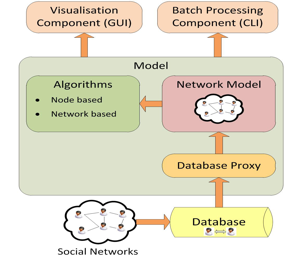
\includegraphics[width=0.4\linewidth]{img/previous_review_system_diagram.png}
	\caption{Figure}
	\label{fig:previous-review-system-diagram}
\end{figure}

As we can see by the design model above, the software was developed using a modular approach with claims of a high degree of extensibility to the existing tool. As C\# .net was used as the base programming language the resulting GUI is of an extremely high standard, with a professional presentation and feel when using it. A criticism however is although the resulting software developed has an extremely well presentable front end, the disadvantage of using a Windows based development environment and programming language is that the software is not transferable between different operating systems. The unfortunate issue with this is that it means the software cannot be run on a Linux or mac based environment. 

 The original design conceived had the algorithms module as a single module with no separation of the type of algorithm to be run or implemented. This was changed in the final design as shown above, so as to provide a greater degree of flexibility for potential researchers using the tool. 

We intend to use the graphical user interface (GUI) in such a way that the interface is essentially a standalone client program. It should be able to access and transmit data and instructions from the client machine to a cluster of machines at the department with the software becoming a lightweight visualisation tool for different social networks or so that it could serve as a dual purpose tool, able to connect and control a cluster of machines or run independently on a single system (e.g. retain all current functionality but incorporate the functionality of a distributed system). The reason for the further development of the previous group's interface is that because the overall look and feel of the GUI is of such a high standard it would be logical to adapt it to the requirements of this project. The database schema is sound and proven to be extremely versatile with the use of Boyce-Codd normal form to reduce data redundancy. This database schema, should the current interface be user-able, is again, another highly desirable  feature of the previous group's work as the ability to switch between a continuous or discrete dataset is implemented extremely well and therefore would allow us to perform research on different types of data such as real time twitter analysis or a batch of data.

There are a few issues to note with this project that have been identified after careful consideration of the requirements of the current project. The main issue that has been identified is the lack of testing in terms of scalability. While the report produced for the social network analysis tool clearly and accurately identifies problems and errors that could arise from use of the tool such as lack of tape ( .i.e. the tape that is played when a user plays the message interaction is empty and therefore would throw an error), node properties incorrect or other errors, there were no reports of scalability testing. This could be perceived to be a serious flaw with the tool as it can clearly been seen in the results of research experiments conducted that the tool may have only been tested up to a total of 7000 nodes. While this is quite a large number, we intend to extend the tools ability to incorporate a large amount of twitter data. This form of data consists mostly of a large number of small clusters with a few edges linking clusters together. With nearly 500 million users on twitter and approximately 250 million active users \cite{twitterusers}, the ability to visualise the network along with its associated temporal data is extremely desirable and with many claims throughout the report as to the ability of the tool to handle large amounts of data, it is a concern that the interface we intend to extend with simple object access protocol (SOAP) functionality could not be suitable for the size of graphs we wish to analyse. However, as the tool can be run in CLI mode ( batch processing mode without the GUI), the claims of large data processing could in fact be true, however, as we intend to push the computational side of the tool onto a cluster for greater processing power and to achieve a distributed system our main concern with the previous tool is that the interface may not be scalable in terms of graph visualisation. 

Another concern is the dependencies structure associated with the design and implementation of the previous tool. As we are only interested in the GUI, it appears substantial changes would need to be made to the tool in order to separate the GUI from the rest of the tool as it is dependant on nearly every other module within the tool. 

While it is clear that the SNA tool was developed to an extremely high standard, the concerns with the previous work in relation to our own is the potential issues with scalability and modular dependency.

There are however, extremely useful sections of the final report produced by the previous group that will in fact prove very useful. For example, they highlight in great detail the operations and possibilities associated with the tool and its database proxy API's developed. This extremely large quantity of high quality specification regarding modules such as the database proxy and the database schema, should prove useful in attempts to dissect the tools structure and code. 
Overall the previous groups work was of a very high standard and the only criticisms that can be put forward apply to issues that they would naturally, given the specification of the SNAT project, not have tested for.
